\chapter{Übersicht}
Über einen konfigurierbaren Crawler können Inhalte von Webseiten bis zu einer bestimmten Tiefe
aus dem Internet in ein Archiv geladen werden. Da dies parallelisiert erfolgen soll,
müssen die Daten nach dem Herunterladen von temporären Verzeichnissen in das gemeinsame
Archivverzeichnis synchronisiert werden. Der aus der URL extrahierte Pfad der Dateien wird
dabei auf das Archiv abgebildet, wobei jede Datei in einen eigenen Archivordner verschoben wird.\\

Beim Crawlvorgang werden zusätzlich Metadaten der heruntergeladenen Dateien erstellt. 
Diese werden in einer Datenbank und als XML-Datei im jeweiligen Archivordner gespeichert.
Die Datenbank soll dabei wieder aus den XML-Daten rekonstruierbar sein. \\ 

Außerdem sollen Filter eingehängt werden können, die bereits in den TMP-Ordnern ungültige Dateien löschen.
Über eine Java-Schnittstelle kann anschließend wieder auf die Daten zugegriffen werden.
Hierzu müssen sich Clients über eine vorgegebene Schnittstelle beim Textarchiv anmelden.
Die Clients werden anschließend bei Änderungen oder neuen Einträgen benachrichtigt und können sich selbstständig über die Schnittstelle einen beliebigen Stand der Daten herunterladen und an Analysetools weitergeben.
Dabei sollen auch neue Dateien den Archivordnern hinzugefügt werden können.
Ebenso sollen die oben genannten XML-Daten um neue Nodes erweiterbar sein.
Zu Vorführzwecken wird ein Testanalysetool erstellt.

\newpage 
% Diagramm

\begin{figure}
	\centering
	\label{spec:dia:moduls}
	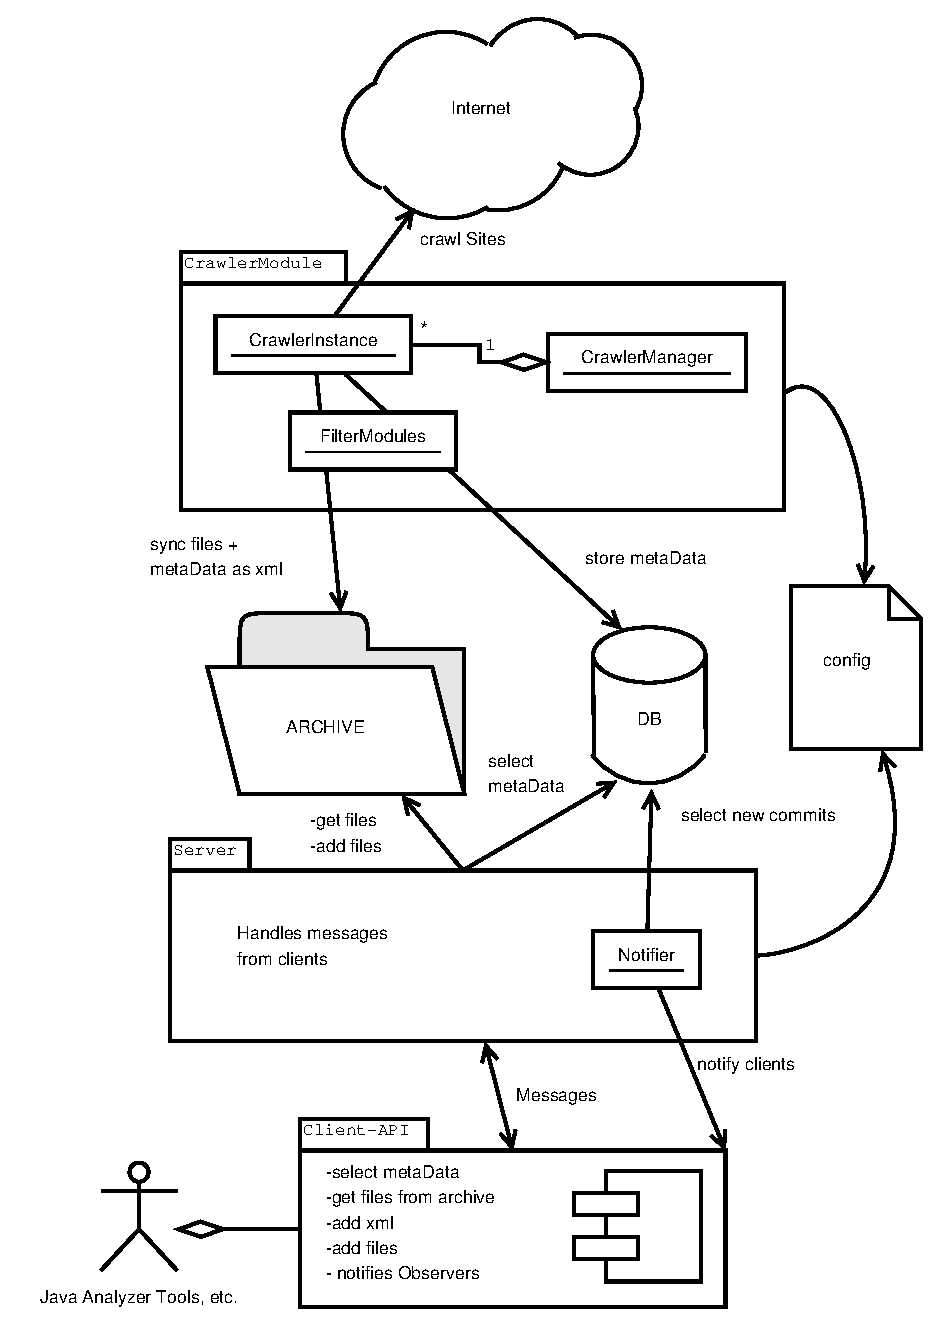
\includegraphics[width=\textwidth]{spec/components.eps}
	\caption{Diagramm: Grundlegendes Design}
\end{figure}
 
